\subsection{カードリスト画面}
カードリスト画面では、木古内で「できること」に着目した観光スポットを写真と紹介文で「カード」という形式にして、それをリスト表示する。一枚のカードに含まれる情報は、そのスポットの写真、キャッチコピーの様なタイトル、紹介文、そしてテキスト編集画面に遷移するボタン、マップ・詳細画面へ遷移するボタン、写真撮影画面へ遷移するボタン、そしてお気に入りボタンといういわゆるブックマーク機能を持つ4つのボタンである。詳しくは表6.1を参照されたい。そしてアプリの画面を図6.1で紹介する。ユーザはキーコ紀行をダウンロードしたらまずこの画面を見て、気になったらそのスポットへ向かう、といったユーザストーリを想定している。使用されている写真は、実際に我々が木古内に行き、撮影したものを使用している。紹介文は、メンバで考えた約70字という制限がついた文である。仮に70字以上の文をカードに表示した場合、カードの見栄えが悪くなってしまうため、見栄えを悪くさせないようにすることを目的として制限した。この画面からは、マップ・詳細画面、写真撮影画面、テキスト編集画面に遷移できる。

\begin{table}[htb]
\centering
\addtocounter{table}{+0}
\caption{カードリストのボタンのアイコンとその意味}
  \begin{tabular}{|c|c|} \hline
    アイコン&意味  \\ \hline 
    \begin{minipage}{10mm}
      \centering
      \scalebox{0.4}{
\includegraphics{pencil.png}}
    \end{minipage} & \parbox{38zw}{テキスト編集画面へ遷移するボタン。}\\  \hline
    \begin{minipage}{10mm}
      \centering
      \scalebox{0.4}{
\includegraphics{pin.png}}
    \end{minipage} &\parbox{38zw}{マップ・詳細画面へ遷移するボタン。}\\ \hline
     \begin{minipage}{10mm}
      \centering
      \scalebox{0.4}{
\includegraphics{camera.png}}
    \end{minipage} & \parbox{38zw}{写真撮影画面へ遷移するボタン。}\\ \hline
	\begin{minipage}{10mm}
      \centering
      \scalebox{0.4}{
\includegraphics{favourites_glay.png}}
    \end{minipage} & \parbox{38zw}{いわゆる「ブックマーク」のようなボタン。ユーザが気に入ったらこのボタンを押し、マップ詳細画面で違うスポットを見たときにでも場所がわかるようになる。}\rule[-6mm]{0mm}{14mm} \\  \hline
  \end{tabular} 
\end{table}

\begin{figure}[htbp]
 \begin{center}
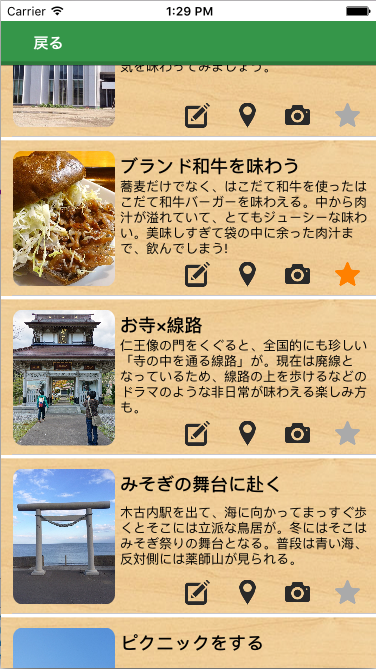
\includegraphics[width=4cm, bb=0 0 303 573]{cardList.png}
 \end{center}
\addtocounter{figure}{+0}
 \caption{カードリスト画面}
 \label{fig:one}
\end{figure}

\bunseki{山川拓也}